\documentclass[draft]{agujournal}
\usepackage{url} 
\usepackage{lineno}
\usepackage[final]{trackchanges} 
\usepackage{soul}
\usepackage{tikz}
\usepackage{booktabs}
\usetikzlibrary{arrows.meta, positioning}
% \usepackage{url}

% \linenumbers
\draftfalse

\journalname{JGR: Earth Surface}


\begin{document}


\title{Urban Heat Island Impact Assessment}

\authors{Daksh Gogna}

\affiliation{1}{Department of Earth Science, IIT Roorkee}

% \correspondingauthor{Daksh Gogna}{daksh\_g@es.iitr.ac.in}

\begin{keypoints}
\item The urban heat island refers to the localized increase in temperature within urban areas compared to their rural surroundings,primarily due to human activities and changes in land cover. 
\item Urban Heat Islands (UHIs) Are Intensifying, Especially in Lower-Income Regions
\item UHIs Have Significant Impacts on Energy Consumption and Public Health
\item Mitigation Strategies Have Evolved Over the Last Three Decades
\end{keypoints}


\begin{abstract}
The Urban Heat Island (UHI) effect, wherein urban areas experience elevated temperatures relative to their rural surroundings, has become a critical issue in the context of global climate change and rapid urbanization. This review synthesizes findings from five contemporary studies examining the multi-dimensional causes, impacts, and mitigation strategies associated with UHIs. These studies span diverse scales—from systematic literature reviews to global satellite-based analyses and city-level energy and mortality modeling—providing a holistic view of UHI phenomena.

A systematic review by Deilami et al. identifies vegetation loss, impervious surface expansion, and seasonal variation as key drivers of UHI. Meanwhile, Yuan et al. reveal a growing disparity in UHI intensity, with low-income countries experiencing the fastest increases in surface urban heat island intensity (SUHII), despite having the least adaptive infrastructure. Anser et al.'s longitudinal econometric analysis of urban China demonstrates that UHI significantly impacts energy consumption, with meteorological and construction variables influencing urban energy demand over nearly five decades.

Akbari and Kolokotsa contribute insights into the evolution of mitigation technologies, documenting the development of high-albedo “cool” materials, vegetative infrastructure, and advanced thermochromic surfaces. These strategies, while effective, remain unevenly deployed across regions. Wang et al. add a vital public health perspective, finding that while UHI increases heat-related mortality, it reduces cold-related deaths significantly, suggesting the need for seasonally adaptive interventions rather than uniform cooling policies.

Taken together, the reviewed literature illustrates that UHIs are not just a function of physical urban structure but are deeply intertwined with economic inequality, energy systems, and public health. The most affected populations—particularly in developing nations—are often the least equipped to respond. Successful mitigation requires integrative approaches that combine remote sensing, data-driven planning, public health insights, and adaptive design. Policy interventions must prioritize equitable solutions that are climate-sensitive and region-specific.

This review concludes that effective UHI mitigation must be interdisciplinary, scalable, and dynamic—addressing both the environmental mechanics and the socio-economic structures that influence urban thermal landscapes. With urban populations growing and temperatures rising, such strategies are essential to ensure sustainable and livable cities worldwide.
\end{abstract}

\section*{Plain Language Summary}
Cities are getting hotter, not just because of climate change but because of how they are built. This is known as the Urban Heat Island (UHI) effect, where urban areas are much warmer than nearby rural regions. Roads, buildings, and pavements absorb more heat than soil and plants, causing cities to heat up during the day and cool down more slowly at night.

This review looked at five major studies on the UHI effect to understand what causes it, who is most affected, and what can be done about it. One study showed that UHI is getting worse faster in low-income countries, where cities are growing rapidly but lack the green spaces and resources needed to keep things cool. Another found that as cities get hotter, they use more electricity for air conditioning, especially in countries like China.

We also looked at ways to reduce the UHI effect, such as using white reflective roofs, planting more trees, or using new materials that change how much heat they absorb depending on the season. However, one study warned that these strategies might have side effects — for example, keeping a city too cool in winter could actually increase deaths from cold.

The big message is that there’s no one-size-fits-all solution. Different cities need different strategies depending on their weather, layout, and income levels. If cities plan smartly — using both science and local knowledge — they can become cooler, safer, and more comfortable for everyone.

\section*{1. Introduction}

The Urban Heat Island (UHI) phenomenon — where urban areas exhibit significantly higher temperatures than adjacent rural zones — has become an increasingly pressing environmental and socio-economic concern in the 21st century. This temperature discrepancy arises from the large-scale replacement of natural land covers like vegetation and soil with impervious surfaces such as asphalt, concrete, and rooftops, which store and radiate heat more efficiently. Rapid urbanization, combined with global climate change, is intensifying the severity and frequency of UHI effects across diverse climatic zones and socio-economic contexts.

Historically, UHIs have been recognized for over a century, but only in the past three decades has systematic scientific inquiry accelerated to understand their dynamics and implications. Cities today host more than half the global population, a figure projected to rise to 68\% by 2050. This demographic shift, particularly pronounced in the developing world, increases the urgency to address urban thermal stress. UHIs exacerbate several urban challenges, including increased energy demands for cooling, deteriorated air quality due to smog formation, amplified health risks such as heat strokes and respiratory illnesses, and reduced livability.

The literature reviewed herein provides a comprehensive understanding of UHI causes, spatial-temporal characteristics, and mitigation strategies. Drawing on five pivotal studies — including global spatial analyses, country-specific econometric evaluations, systematic reviews, and mortality modeling — this review aims to synthesize current insights into UHI intensification trends, technological and natural countermeasures, and implications for urban planning and public health. These findings collectively inform a multidimensional perspective on the UHI problem, highlighting the need for evidence-based, adaptive, and equity-driven solutions.

\section*{2. Data and Methodologies}

The selected body of literature employs a rich blend of data types and analytical methodologies to investigate the Urban Heat Island (UHI) phenomenon. These studies span global to regional scales, employing remote sensing, econometric analysis, statistical modeling, and simulation-based assessments. Each methodology contributes uniquely to the collective understanding of UHI causality, variability, and response strategies.

\textbf{Remote Sensing and Land Surface Temperature (LST) Derivation:} Deilami et al. (2018) conducted a systematic review of 75 UHI-focused studies, identifying satellite-derived land surface temperature (LST) as the most commonly used proxy for detecting UHI intensity. Approximately 54\% of the studies utilized Landsat TM data, 34\% used Landsat ETM+, and 28\% used MODIS imagery. Analytical techniques employed included land cover classification via indices (46\%), supervised classification (17\%), and regression modeling — with Ordinary Least Squares (OLS) being the most frequent.

\textbf{Econometric and Statistical Models:} Anser et al. (2025) used the Generalized Method of Moments to evaluate how urban form, meteorology, and materials affected China’s energy consumption (1975–2022). Granger causality identified bidirectional links between land use and energy use.

\textbf{Health Impact Modeling and Machine Learning:} Wang et al. (2025) analyzed mortality data across more than 3,000 global cities, integrating it with climate, socio-economic, and LST datasets. They implemented a machine learning framework to examine non-linear relationships between temperature changes and mortality. The study assessed the dual nature of UHI impacts — both aggravating heat-related deaths and alleviating cold-related mortality.

\textbf{Technology Review:} Akbari and Kolokotsa (2016) adopted a qualitative meta-review methodology to assess the evolution of cool materials and green infrastructure over three decades. Their work catalogs mitigation techniques ranging from cool roofs and pavements to thermochromic surfaces and directionally reflective materials.

These methodological approaches provide both depth and breadth, enabling a multi-scale, multi-factorial understanding of UHI causes and mitigation effectiveness.

\section*{3. Results and Synthesis}

The reviewed literature presents a robust set of findings on the dynamics, disparities, and implications of the Urban Heat Island (UHI) effect. These findings span physical mechanisms, socio-economic variations, energy consumption trends, mortality impacts, and technological countermeasures.

\subsection*{3.1 Physical and Spatial Drivers}

Deilami et al. (2018) demonstrated that vegetation cover (44\%), built-up areas (28\%), seasonality (33\%), population density (14\%), and water bodies (12\%) were consistently cited as major factors influencing UHI intensity. Their review found that UHI effects were generally more pronounced during summer and nighttime due to reduced longwave radiation dissipation and higher thermal inertia of urban surfaces.

\subsection*{3.2 Socioeconomic Disparities}

Yuan et al. (2025) conducted the first global gridded comparison of SUHII trends by income level. While high-income countries (e.g., U.S., China) had large areas affected by UHI, the most intense growth in SUHII occurred in low-income countries. Between 2003 and 2018, SUHII increased on average by 0.033°C/year in low-income countries during daytime, compared to 0.015°C/year in high-income ones. During nighttime, the strongest increases were observed in lower-middle-income countries, reaching 0.019°C/year.

\begin{table}[h]
\centering
\caption{\textbf{Table 1.} SUHII Trends by Income Group (2003--2018)}
\begin{tabular}{@{}lcc@{}}
\toprule
\textbf{Income Group} & \textbf{Daytime SUHII (°C/year)} & \textbf{Nighttime SUHII (°C/year)} \\
\midrule
High-income            & 0.015                          & 0.010                             \\
Upper-middle-income    & 0.020                          & 0.015                             \\
Lower-middle-income    & 0.025                          & 0.019                             \\
Low-income             & 0.033                          & 0.014                             \\
\bottomrule
\end{tabular}
\label{tab:suhii_trends}
\end{table}

\subsection*{3.3 Energy Consumption and Efficiency}

Anser et al. (2025) analyzed China’s urban energy patterns from 1975 to 2022. The study found that urban form, meteorological factors, land use, and construction materials significantly influenced energy demand. Meteorological factors alone accounted for a 12.62\% variation in energy consumption, while land use and building materials accounted for 3.6\% and 1.4\%, respectively. Renewable energy interventions showed a 1.5\% reduction in conventional urban energy usage.

Causality tests demonstrated that building materials, land use, and urban form influence each other bidirectionally. Projected energy consumption indicates that without adaptive interventions, urban areas may see increased demand through 2030, especially in construction-dense regions.

\subsection*{3.4 Technological and Natural Mitigation Strategies}

Akbari and Kolokotsa (2016) evaluated UHI mitigation efforts spanning three decades. Key interventions include:
\begin{itemize}
  \item \textbf{Cool Roofs and Pavements:} These use high albedo materials to reflect solar radiation, reducing surface temperatures by up to 30°C. White coatings, light-colored tiles, and advanced reflective pigments were widely adopted in the U.S. and EU.
  \item \textbf{Urban vegetation:} Urban greenery increases latent heat flux and reduces surface temperature. Green roofs, vertical gardens, and permeable pavements are now used in various climate zones.
  \item \textbf{Directional and Thermochromic Materials:} Directionally Reflective Materials (DRMs) reduce heat absorption in summer but retain heat in winter. Thermochromic materials change reflectivity based on temperature, though photo-degradation remains a hurdle for long-term outdoor use.
\end{itemize}
The findings emphasize that combining cool materials with vegetative strategies achieves the highest impact, especially when tailored to local climates.

\subsection*{3.5 Dual Mortality Effects of UHI}

Wang et al. (2025) revealed that UHI effects have a paradoxical impact on mortality. While UHIs increase heat-related deaths, especially during heatwaves in tropical cities, they also substantially reduce cold-related mortality in colder regions. Globally, cold-related mortality reductions were found to be over four times greater than heat-related mortality increases, suggesting that UHIs provide a net mortality benefit in many contexts.

However, widespread cooling interventions like increased albedo or greenery may unintentionally raise cold mortality in temperate regions. A solution proposed is seasonal albedo modulation, adjusting reflectivity by season to maintain benefits year-round.

\subsection*{3.6 Summary Schematic}
Below is a simplified schematic of interlinked UHI factors and impacts, synthesized from the five studies:

\begin{figure}[h]
\centering
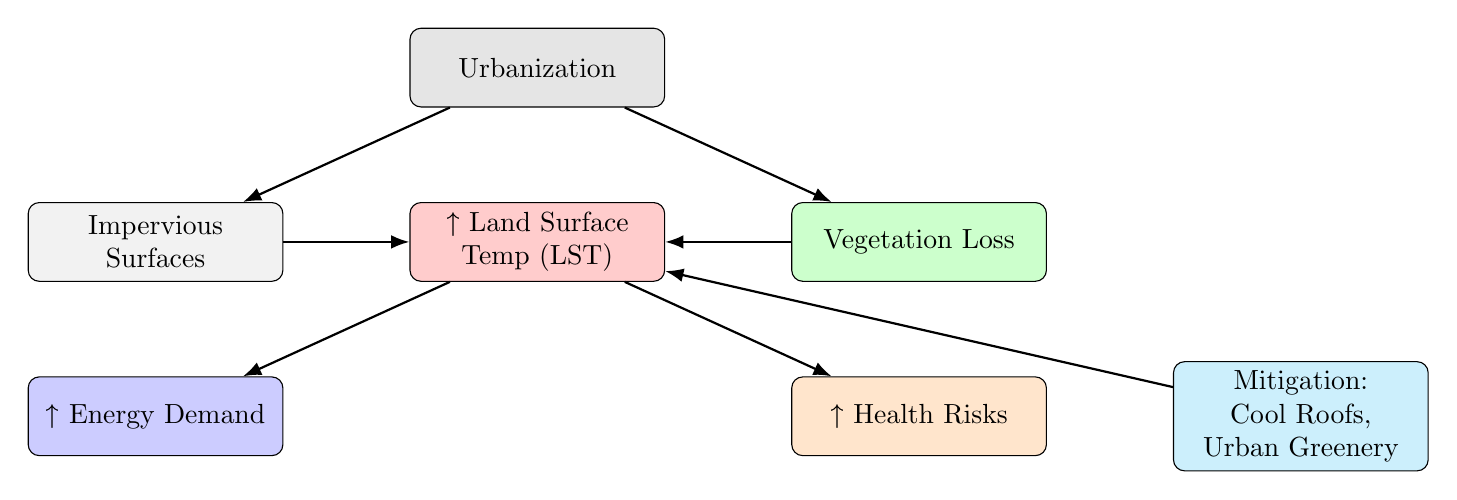
\begin{tikzpicture}[
  node distance=1.2cm and 1.6cm,
  box/.style={rectangle, draw, rounded corners, minimum height=1cm, text centered, text width=3cm, fill=gray!10},
  arrow/.style={-{Latex}, thick}
]

\node[box, fill=gray!20] (urban) {Urbanization};
\node[box, below left=of urban] (impervious) {Impervious Surfaces};
\node[box, below right=of urban, fill=green!20] (veg_loss) {Vegetation Loss};
\node[box, below=of urban, fill=red!20] (lst) {↑ Land Surface Temp (LST)};
\node[box, below left=of lst, fill=blue!20] (energy) {↑ Energy Demand};
\node[box, below right=of lst, fill=orange!20] (health) {↑ Health Risks};
\node[box, right=of health, fill=cyan!20] (mitigation) {Mitigation: \\ Cool Roofs, \\ Urban Greenery};

\draw[arrow] (urban) -- (impervious);
\draw[arrow] (urban) -- (veg_loss);
\draw[arrow] (impervious) -- (lst);
\draw[arrow] (veg_loss) -- (lst);
\draw[arrow] (lst) -- (energy);
\draw[arrow] (lst) -- (health);
\draw[arrow] (mitigation) -- (lst);

\end{tikzpicture}
\caption{Flowchart summarizing UHI causes, effects, and mitigation interventions.}
\label{fig:uhi_summary}
\end{figure}

\section*{4. Discussion}

The synthesis of findings across the five reviewed papers reveals three central themes: (1) the multifaceted drivers of UHI, (2) global inequity in exposure and mitigation capacity, and (3) the importance of adaptive, context-sensitive solutions.

\subsection*{4.1 Complexity of Drivers and Feedback Loops}
Urban Heat Islands are not merely a function of land cover change but result from the interplay of physical, socio-economic, and technological systems. Vegetation loss, land sealing, and building density elevate local temperatures. This, in turn, increases cooling energy demand, creating feedback loops of waste heat and emissions. Anser et al. (2025) and Deilami et al. (2018) both emphasized how urban form and meteorology interact to affect both surface temperature and energy consumption. These feedbacks are non-linear, demanding integrated urban planning approaches.

The introduction of directional reflective materials and thermochromic surfaces, as reported by Akbari and Kolokotsa (2016), shows promise in breaking some of these feedback cycles. However, adoption remains low outside developed countries due to technical complexity, cost, and lack of policy support.

\subsection*{4.2 Disproportionate Burden on Lower-Income Countries}
Yuan et al. (2025) compellingly demonstrated that the fastest intensification of SUHII occurs in low- and lower-middle-income nations — precisely where adaptive capacity is weakest. These regions often lack sufficient vegetation, climate-sensitive zoning regulations, and capital for retrofitting urban infrastructure.

What’s more, Wang et al. (2025) highlighted a paradox: cities in temperate zones may unintentionally harm public health by implementing universal cooling strategies. This underscores the danger of “one-size-fits-all” solutions and the need for thermal policies that respect both seasonal and geographic variability.

\subsection*{4.3 Need for Seasonal and Spatial Adaptation}
The divergence between cooling benefits in tropical cities and warming benefits in colder climates indicates the need for seasonally tuned UHI interventions. Static measures — such as permanently high-albedo surfaces — may reduce summer heat but could amplify winter cold risks. Instead, modifiable elements (e.g., switchable coatings or deciduous vegetation) could offer dynamic thermal regulation. This has profound implications for design standards in temperate and high-latitude cities.

\subsection*{4.4 Interdisciplinary Integration}
Finally, a recurring theme is the need for cross-sectoral cooperation. Urban planners, climate scientists, public health experts, and economists must co-develop strategies that not only mitigate UHI but also enhance sustainability, equity, and liveability. The data-driven modeling by Wang et al. and Anser et al. demonstrates how combining climatological and socio-economic datasets can guide more targeted, efficient interventions.

\section*{5. Conclusion}

The Urban Heat Island (UHI) effect represents one of the most urgent and multifactorial challenges facing modern cities. It emerges from a confluence of urban morphology, land cover transformation, meteorological dynamics, socio-economic disparities, and policy limitations. This review, drawing from five high-quality studies, has demonstrated that the causes, impacts, and solutions to UHI vary dramatically across spatial and temporal scales.

Key findings affirm that urbanization intensifies surface temperatures due to increased impervious surfaces, reduced vegetation, and anthropogenic heat release. Deilami et al. (2018) highlighted these drivers through a systematic review, while Anser et al. (2025) confirmed their downstream effects on urban energy consumption in China. Their work emphasizes that mitigation strategies must consider urban layout, construction materials, and local climate variables.

Yuan et al. (2025) revealed a growing inequality in UHI exposure: low-income countries are experiencing the fastest increases in SUHII but possess the least adaptive infrastructure. Akbari and Kolokotsa (2016) provided a long-term perspective on available mitigation tools — from cool roofs and reflective materials to urban vegetation. Yet, uptake remains limited in vulnerable regions due to institutional and economic barriers.

Perhaps most critically, Wang et al. (2025) exposed a duality in UHI health impacts — while increasing heat-related mortality, UHIs significantly reduce cold-related deaths, especially in temperate climates. This insight calls for a paradigm shift toward seasonally adaptive UHI interventions rather than blanket solutions.

In closing, cities must respond to UHI with data-driven, climate-sensitive, and equity-centered policies. Investments should target vulnerable geographies, and policies must integrate UHI mitigation into housing, transportation, and energy systems. Dynamic solutions — such as seasonal albedo modulation and responsive green infrastructure — offer promising paths forward.

With urbanization accelerating worldwide, the time to embed UHI resilience into city planning is now. The lessons drawn from these studies form a critical knowledge base for informed action across disciplines, sectors, and borders.


\acknowledgments
I would like to appreciate the vision and structured course planning of the Department of Earth Sciences, IIT Roorkee to introduce a course on a less known but greatly necessary computer language \LaTeX among students for writing and publishing research papers and thesis reports in the first year itself. I would also like to extend my heartfelt gratitude to Professor Kamal for teaching us the subject and supervising our works.  

\bibliography{uhiagu}
\cite{3decades}
\cite{energyconsumption}
\cite{uhireview}
\cite{uhiincome}
\cite{uhimortality}

\end{document}



